\chapter{ Simulation results of a two-stage single-ended symmetric OTA}
\label{ch:chap5}


\section{Open Loop Case of a two-stage single-ended symmetric OTA  (Without Feedback)}
    \begin{figure}[h]
        \centering
           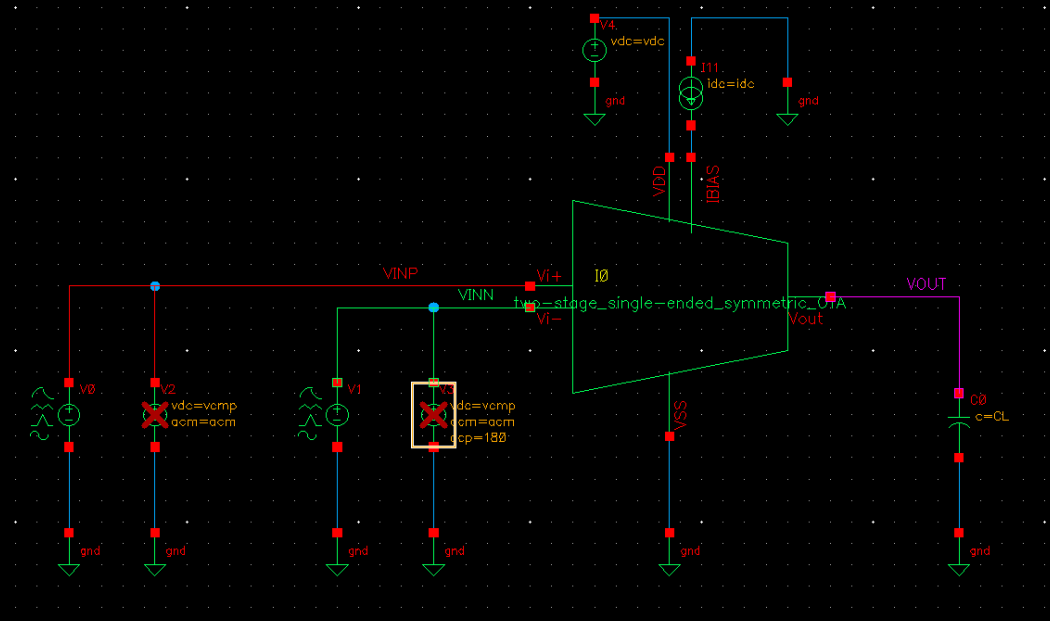
\includegraphics[width=1\textwidth]{images/two_stage_ota_open.png}
        \caption{A two-stage single-ended symmetric OTA - open loop case}
        \label{fig: }
    \end{figure}
    

\subsection{Transient Analysis Setup}

\begin{table}[h]
    \centering
    \captionsetup{justification=centering} % Ensure centering
    \caption*{\textbf{Transient Analysis Parameters of a two-stage single-ended symmetric OTA  - open loop case}} % Centered caption
    \begin{tabular}{l l l l}
        \toprule
        Terminal & Property & Symbol & Value \\
        \midrule
        Vin+ & Delay Time & vinp delay & 1 µs \\
        Vin+ & Zero Value & vinp zero & 1 V \\
        Vin+ & One Value & vinp one & 0 V \\
        Vin+ & Period of Waveform & vinp period & 20 µs \\
        Vin+ & Rise Time & vinp rise & 100 ns \\
        Vin+ & Fall Time & vinp fall & 100 ns \\
        Vin- & Delay Time & vinn delay & 1 µs \\
        Vin- & Zero Value & vinn zero & 0 V \\
        Vin- & One Value & vinn one & 1 V \\
        Vin- & Period of Waveform & vinn period & 20 µs \\
        Vin- & Rise Time & vinn rise & 100 ns \\
        Vin- & Fall Time & vinn fall & 100 ns \\
        \bottomrule
    \end{tabular}
    \label{tab:transient_analysis}
\end{table}


\subsection{Slew Rate Analysis}
The slew rate is calculated using the following expression in Cadence:


\begin{equation}
\text{slewRate} \left( v("/VOUT", \text{?result} = "tran"), 0, \text{nil}, 1, \text{nil}, 10, 90, \text{nil}, "time" \right)
\end{equation}

The obtained slew rate is:

\begin{equation}
\text{Slew Rate} = 11.5636\, \text{V/µs}
\end{equation}

The slew rate (SR) is calculated based on the rising edge, representing the maximum rate of change of the output voltage ($V_{OUT}$):


\textbf{Manual Calculation}


    \begin{figure}[h]
        \centering
           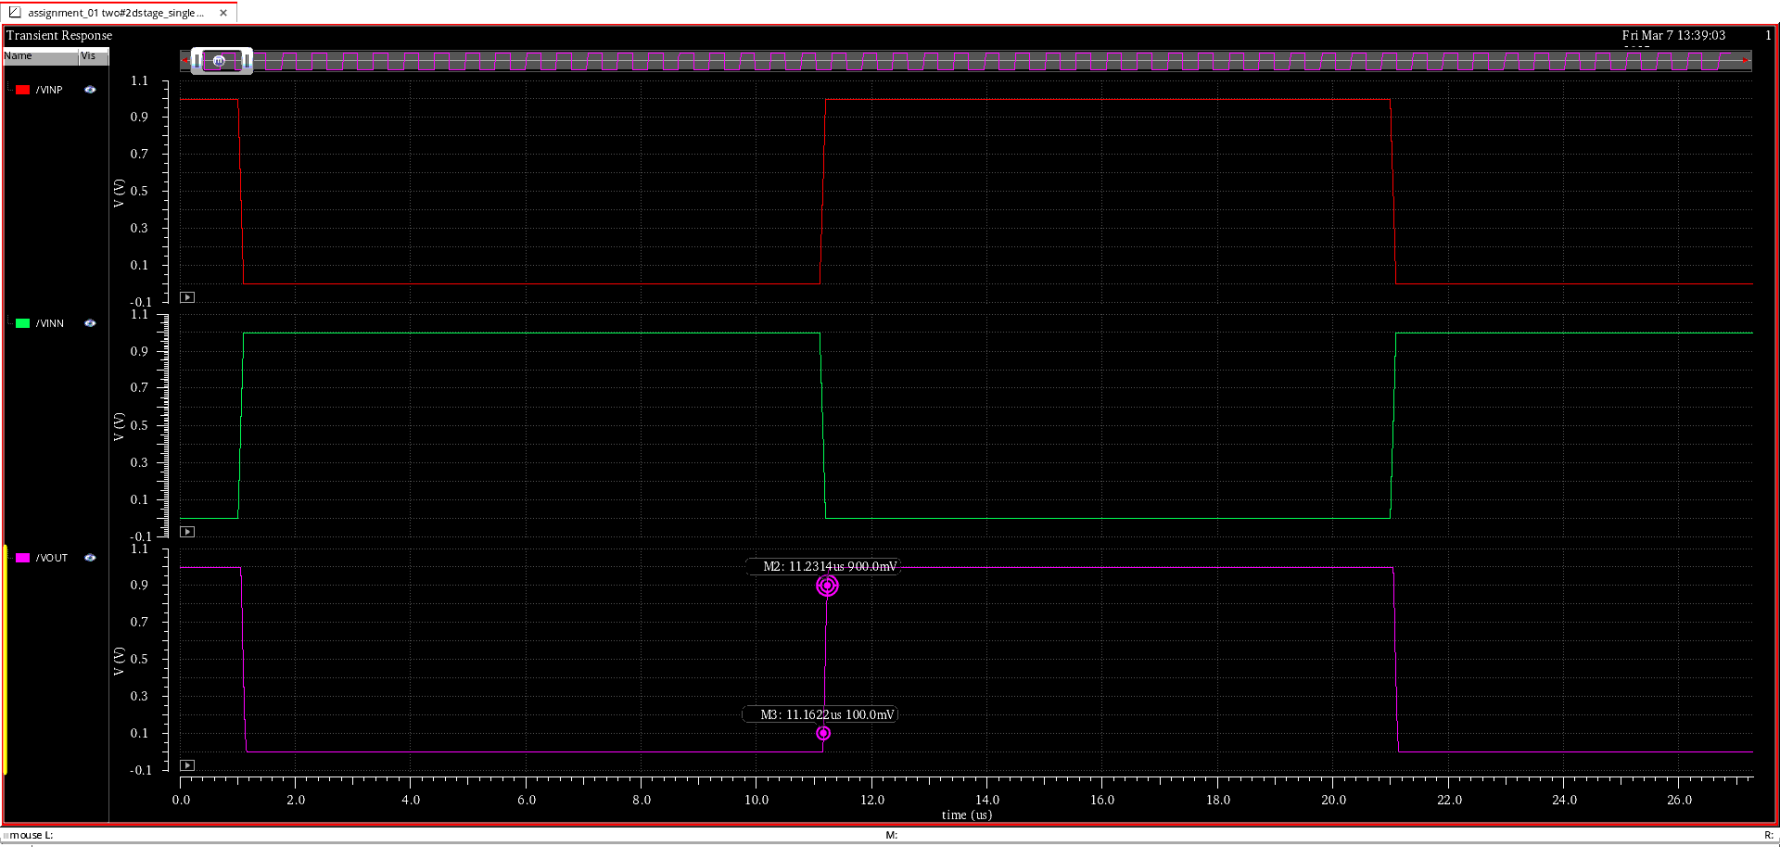
\includegraphics[width=1\textwidth]{images/two_stage_ota_open_slew.png}
        \caption{Slew Rate Analysis Open Loop of a two-stage single-ended symmetric OTA  }
        \label{fig: }
    \end{figure}

\begin{equation}
    SR = \frac{\Delta V_{OUT}}{\Delta t}
\end{equation}

From the transient response, $V_{OUT}$ transitions from 100 mV to 900 mV over 11.1622 $\mu$s to 11.2314 $\mu$s:

\begin{equation}
    SR = \frac{900 \times 10^{-3} - 100 \times 10^{-3}}{11.2314 \times 10^{-6} - 11.1622 \times 10^{-6}}
\end{equation}

\begin{equation}
    SR = \frac{800 \times 10^{-3}}{0.0692 \times 10^{-6}}
\end{equation}

\begin{equation}
    SR \approx 11.5606 \text{ V/} \mu s
\end{equation}


\subsection{AC Analysis Setup}
For the AC analysis, a 500 mV DC voltage with a 1 V AC signal, incorporating two signals with 0$^\circ$ and 180$^\circ$ phase shifts, was applied.


    \begin{figure}[h]
        \centering
           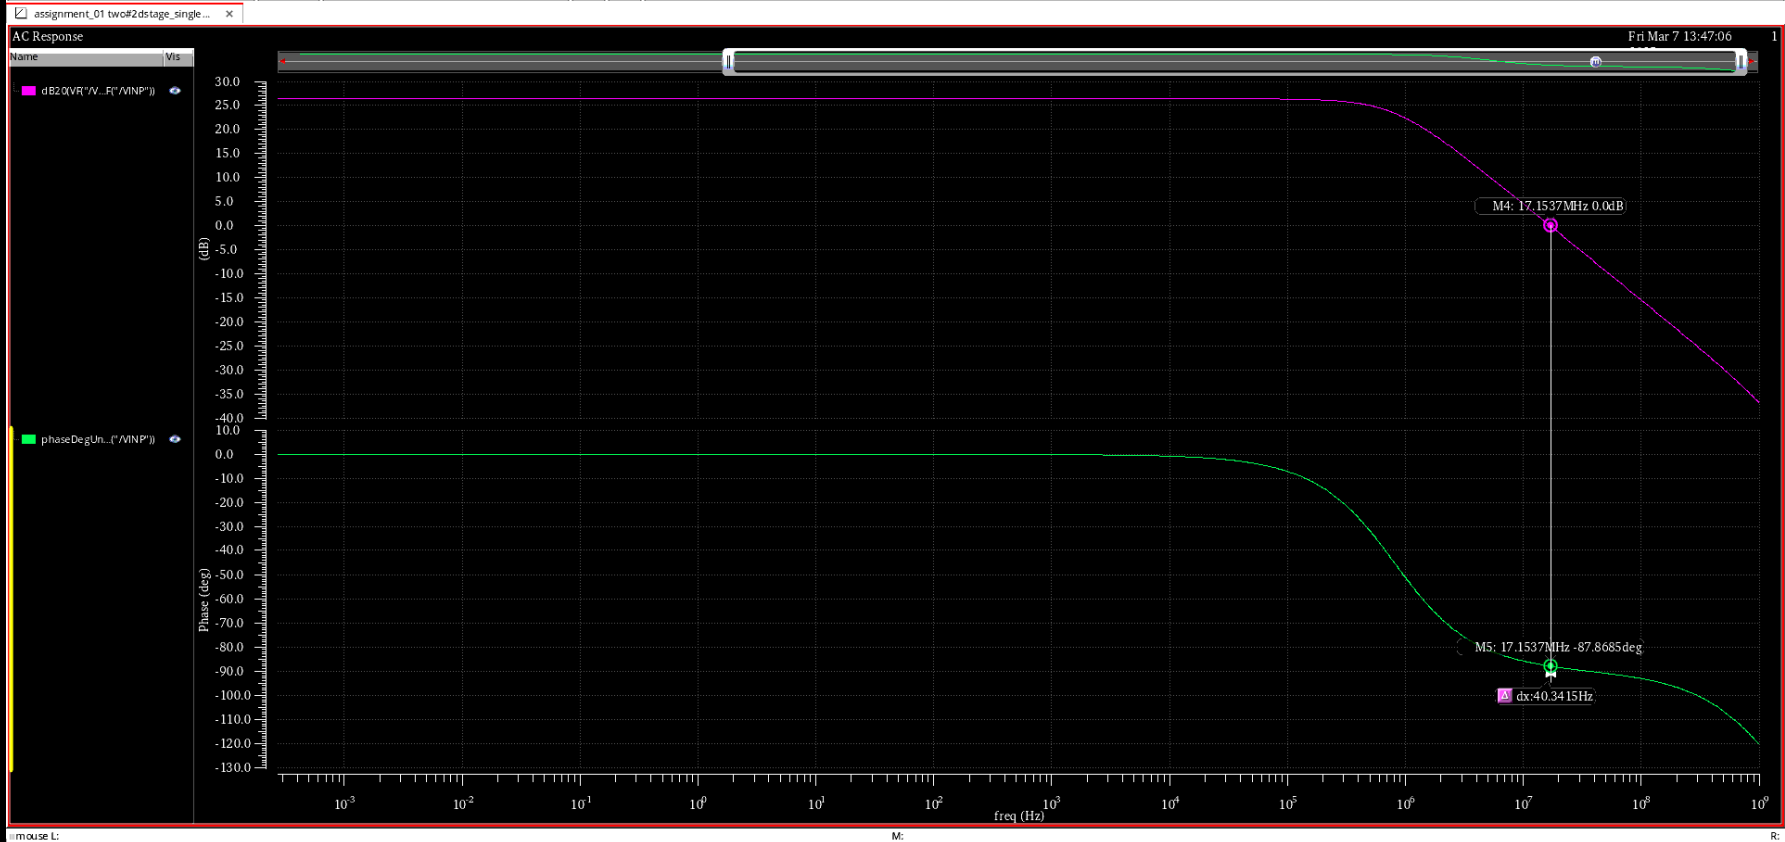
\includegraphics[width=1\textwidth]{images/two_stage_ota_open_ac.png}
        \caption{Slew Rate Analysis Open Loop of a two-stage single-ended symmetric OTA }
        \label{fig: }
    \end{figure}
\newpage
\subsection{AC Analysis Results}
The AC analysis results are derived from the frequency response plot:

\begin{itemize}
    \item \textbf{DC Gain}: Approximately 26.4813 dB at 1 nHz, below the specification of $\geq$ 40 dB.
    \item \textbf{Unity Gain Bandwidth (UGBW)}: Approximately 17.1537 MHz, below the specification of $\geq$ 20 MHz.
    \item \textbf{Phase Margin (PM)}: At 17.1537 MHz, the phase is $-87.8685^\circ$, giving:
    \begin{equation}
        PM = 180^\circ - 87.8685^\circ \approx 92.1315^\circ
    \end{equation}
    This exceeds the specification of $>$ 45$^\circ$.
\end{itemize}

\begin{table}[h]
    \centering
    \captionsetup{justification=centering} % Ensure centering
    \caption*{\textbf{Comparison of Open Loop Results with Design Specifications of a two-stage single-ended symmetric OTA }} % Centered caption
    \begin{tabular}{l c c c}
        \toprule
        \textbf{Parameter} & \textbf{Design Specification} & \textbf{Obtained Value} & \textbf{Unit} \\
        \midrule
        Open-loop DC Gain & $\geq$100 (40 dB) & 26.4813 & dB \\
        Unity Gain Frequency & $\geq$20 MHz & 17.1537 & MHz \\
        Phase Margin & $>$45$^\circ$ & 92.1315 & $^\circ$ \\
        Slew Rate & $>$10 V/$\mu$s & 11.5606 & V/$\mu$s \\
        \bottomrule
    \end{tabular}
\end{table}

\newpage
\section{Closed Loop of a two-stage single-ended symmetric OTA  (With Unity Gain Feedback)}
    \begin{figure}[h]
        \centering
           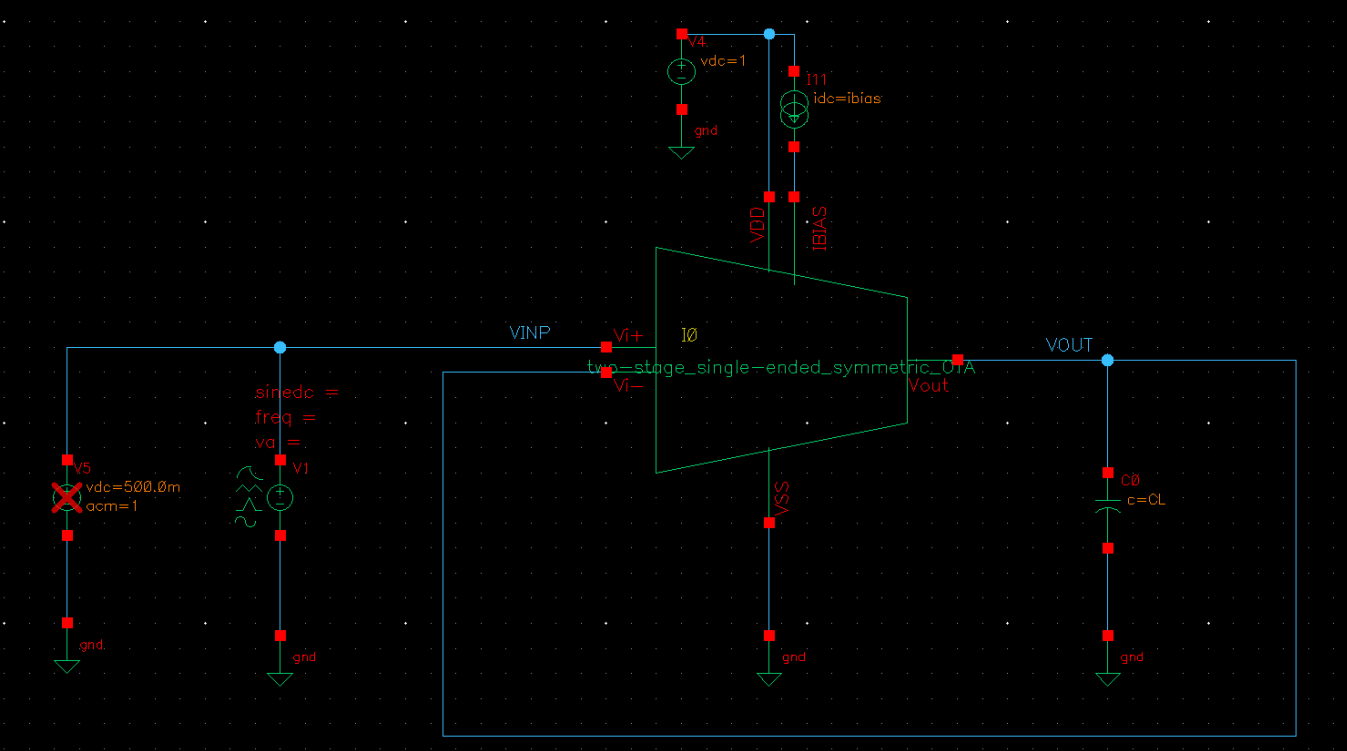
\includegraphics[width=1\textwidth]{images/two_stage_ota_close.png}
        \caption{closed Loop of a two-stage single-ended symmetric OTA  }
        \label{fig: }
    \end{figure}
    
\subsection{Transient Analysis Setup}

\begin{table}[h]
    \centering
    \captionsetup{justification=centering} % Ensure centering
    \caption*{\textbf{Transient Analysis Parameters of a two-stage single-ended symmetric OTA - Closed loop}} % Centered caption
    \begin{tabular}{l l l l}
        \toprule
        Terminal & Property & Symbol & Value \\
        \midrule
        Vin+ & Delay Time & vinp delay & 1 µs \\
        Vin+ & Zero Value & vinp zero & 1 V \\
        Vin+ & One Value & vinp one & 0 V \\
        Vin+ & Period of Waveform & vinp period & 20 us \\
        Vin+ & Rise Time & vinp rise & 100 ns \\
        Vin+ & Fall Time & vinp fall & 100 ns \\
        \bottomrule
    \end{tabular}
    \label{tab:transient_analysis}
\end{table}


\subsection{Slew Rate Analysis}
    \begin{figure}[h]
        \centering
           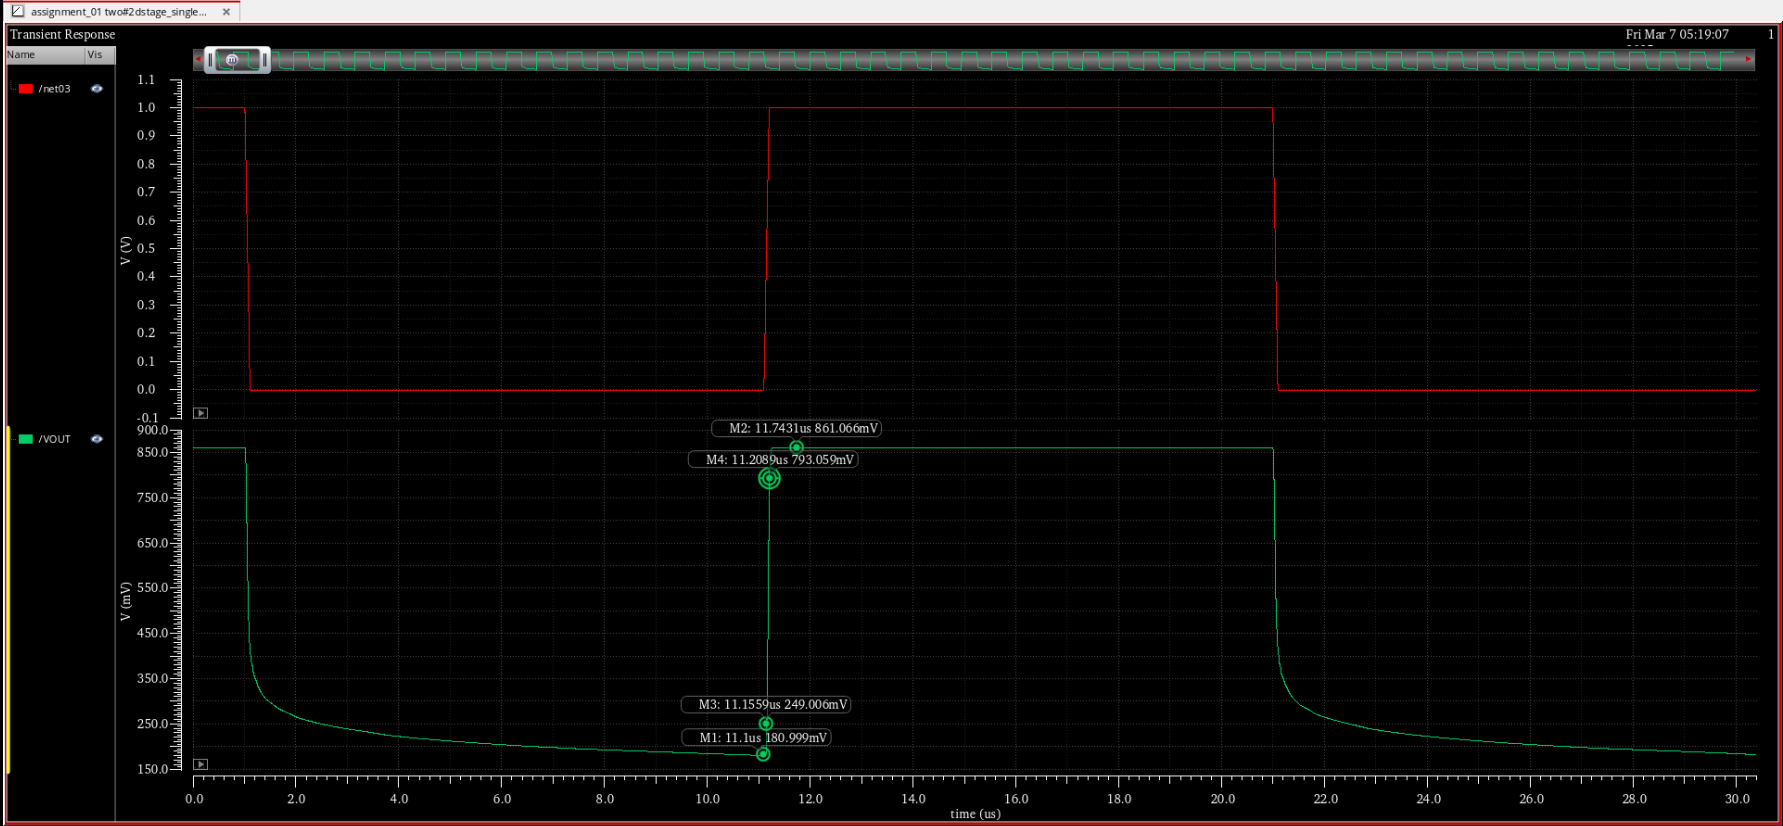
\includegraphics[width=1\textwidth]{images/two_stage_ota_close_slew.png}
        \caption{Slew Rate Analysis for closed Loop of a two-stage single-ended symmetric OTA  }
        \label{fig: }
    \end{figure}

The transient response is driven by a pulse input with the following parameters:

\begin{equation}
    SR = \frac{\Delta V_{OUT}}{\Delta t}
\end{equation}

From the transient response, $V_{OUT}$ transitions from 249.006 mV to 793.059 mV over 11.1559 $\mu$s to 11.2089 $\mu$s:

\begin{equation}
    SR = \frac{793.059 \times 10^{-3} - 249.006 \times 10^{-3}}{ 11.2089  \times 10^{-6} -  11.1559 \times 10^{-6}}
\end{equation}

\begin{equation}
    SR = \frac{544.053 \times 10^{-3}}{0.053 \times 10^{-6}}
\end{equation}

\begin{equation}
    SR \approx 10.2651 \text{ V/} \mu s
\end{equation}

\subsection{AC Analysis Setup}


For the AC analysis, a 500 mV DC voltage with a 1 V AC signal was applied to the $V_{INP}$ terminal.
    \begin{figure}[h]
        \centering
           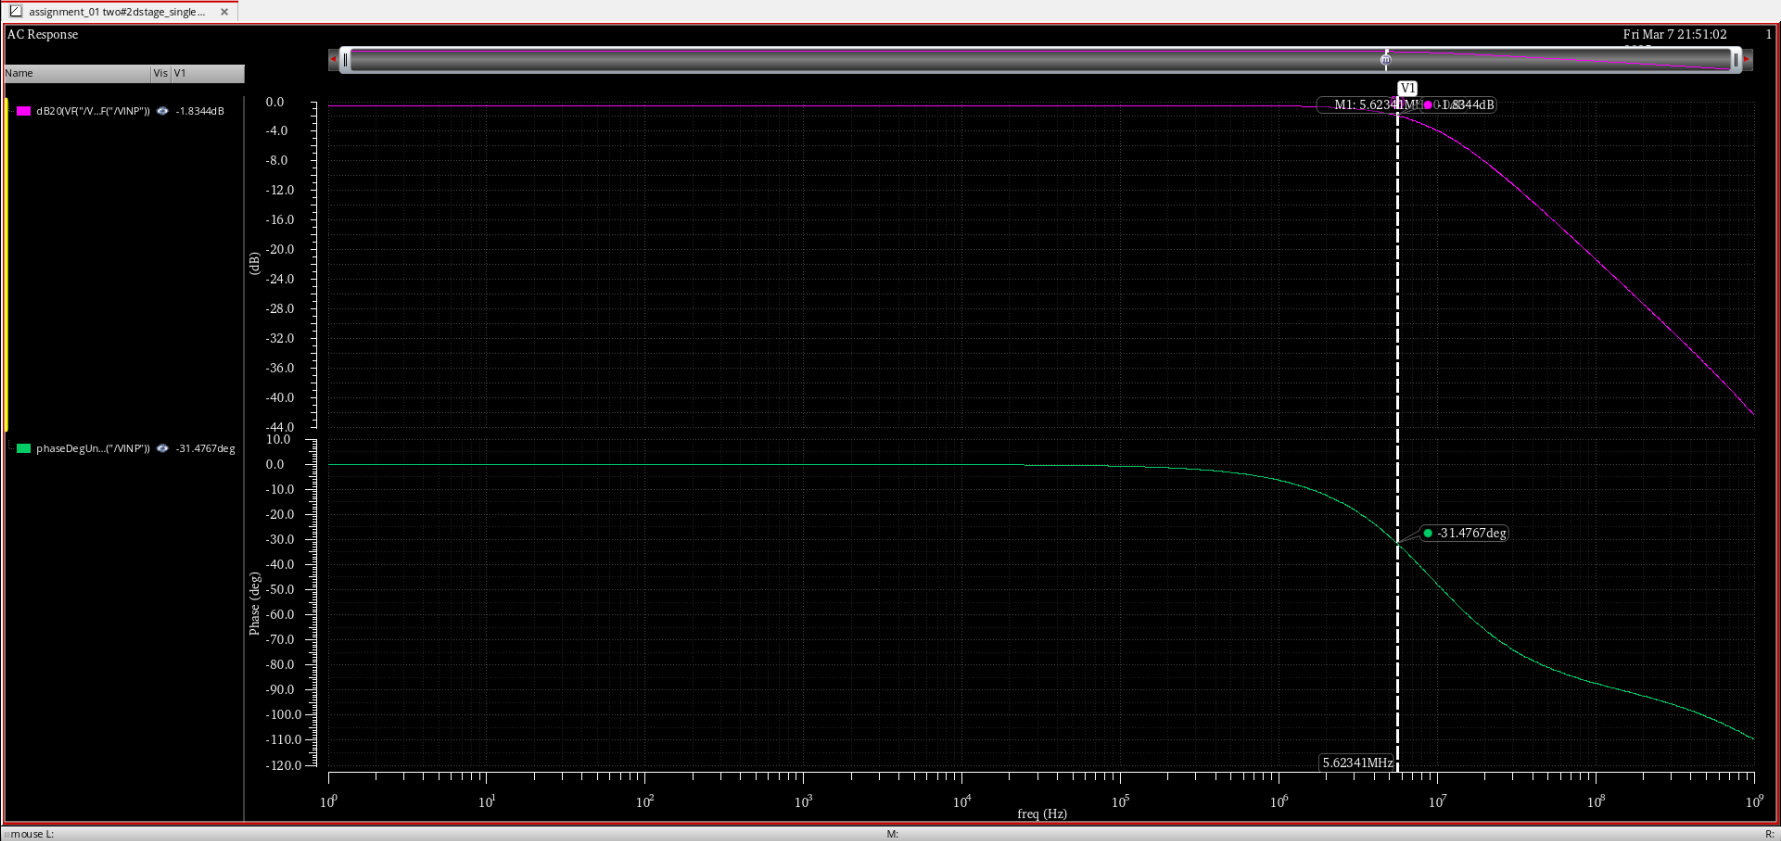
\includegraphics[width=1\textwidth]{images/two_stage_ota_close_ac.png}
        \caption{AC Analysis for closed Loop of a two-stage single-ended symmetric OTA }
        \label{fig: }
    \end{figure}






\section{ A(table of) comparison between design/simulation results and a brief explanation}





    \begin{figure}[h]
        \centering
           \includegraphics[width=0.35\textwidth]{}
        \caption{}
        \label{fig: }
    \end{figure}

\endinput